\section{Physical Layer}
\label{sec:osi_physical}

\vfill
\section*{tl;dr}
The first layer of the OSI model is responsible for the physical transmission of data over a medium. It defines the hardware elements involved in the communication process, such as cables, switches, and network interface cards (NICs). The physical layer ensures that data is transmitted as raw bits over a physical medium, without any concern for the content or meaning of those bits.

The Physical Layer is responsible for:
\begin{itemize}
    \item Converting bits to electrical, optical, or radio signals
    \item Defining voltage levels, timing, and physical data rates
    \item Specifying physical connectors and cable types
    \item Managing the physical topology of the network
    \item Synchronizing transmission between devices
\end{itemize}


\vfill
\subsection*{How does data exchange work? $\star$}
On a physics level, data exchange is about sending and receiving bits over some medium. 

This is done by converting the bits into electrical, optical, or radio signals. Electricity flows through wires, light pulses travel through fiber optics, and radio waves propagate through the air.


In essence, all of them boil down to a similar process: a change in some physical property (voltage, light intensity, or electromagnetic field) that can be detected by the receiving device, such that it can decode the signal back into bits. The process of converting bits into signals is called \textbf{modulation}, and the reverse process is called \textbf{demodulation}, while the process of converting bits into a specific format for transmission is called \textbf{encoding}.

\vfill
\newpage
\vfill
Let's look at a simple example of a 1-bit ADC (Analog to Digital Converter) that converts a voltage level into a bit value:

% assets/osi/physical/adc_plot.png
\begin{figure}[h]
    \centering
    \includegraphics[width=.5\textwidth]{assets/osi/physical/adc_plot.png}
    \caption{Example of a 1-bit ADC converting voltage levels to bits}
    \label{fig:adc_plot}
\end{figure}

However, as you can probably guess, there are infinite ways for us to interpret this graph. It could correspond to \texttt{1010} or \texttt{1111000011110000} and so on. 
This is where clock signals come into play, which help us determine when to sample the signal and how to interpret it.

\vfill
\subsection*{Let's talk timing $\star$}
Clocks or timing signals are present in all hardware communication. 

The idea is to ensure that both sender and receiver are synchronized in their understanding of when bits are being sent and received. 

As an analogy, think of a dance where both partners need to be in sync to perform the moves correctly. If one partner is out of sync, the dance will look awkward and may not work at all.

\begin{figure}[h]
    \centering
    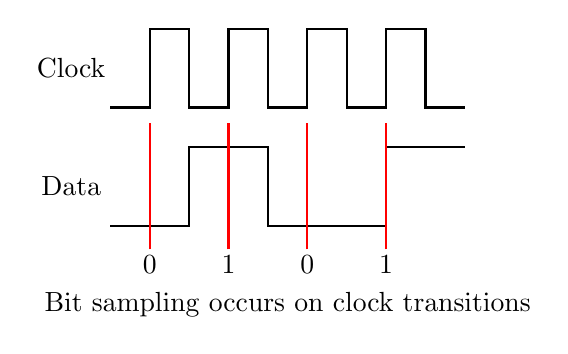
\begin{tikzpicture}
        % Clock signal
        \draw[thick] (0,2) -- (0.5,2) -- (0.5,3) -- (1,3) -- (1,2) -- (1.5,2) -- (1.5,3) -- (2,3) -- (2,2) -- (2.5,2) -- (2.5,3) -- (3,3) -- (3,2) -- (3.5,2) -- (3.5,3) -- (4,3) -- (4,2) -- (4.5,2);
        \node at (-0.5,2.5) {Clock};
        
        % Data signal
        \draw[thick] (0,0.5) -- (1,0.5) -- (1,1.5) -- (2,1.5) -- (2,0.5) -- (3.5,0.5) -- (3.5,1.5) -- (4.5,1.5);
        \node at (-0.5,1) {Data};
        
        % Sampling points
        \foreach \x in {0.5,1.5,2.5,3.5}
            \draw[red,thick] (\x,0.2) -- (\x,1.8);
        
        % Bit values
        \node at (0.5,0) {0};
        \node at (1.5,0) {1};
        \node at (2.5,0) {0};
        \node at (3.5,0) {1};
        
        % Labels
        \node at (2.25,-0.5) {Bit sampling occurs on clock transitions};
    \end{tikzpicture}
    \caption{Example rising edge clock synchronization}
    \label{fig:clock_sync}
\end{figure}
\vfill
\newpage
\section*{Transmission Media}
Different physical media carry the signals that transport our data across networks:

\subsection*{Guided Media}
Guided media confines signals to a specific path (literally "guided" along a cable or fiber). This includes:

\subsubsection*{Twisted Pair Cable}
You probably know this one well, as you find it in most local area networks (LANs) and telephone systems. It consists of pairs of insulated copper wires twisted together to reduce electromagnetic interference.

\begin{minipage}{0.6\textwidth}

UTP (Unshielded Twisted Pair) is the most common type, but there are also shielded variants like STP (Shielded Twisted Pair) and F/UTP (Foiled Unshielded Twisted Pair).

\end{minipage}
\hfill
\begin{minipage}{0.3\textwidth}
    \centering
    \includegraphics[width=\textwidth]{assets/osi/physical/f-utp.png}
    \caption{F-UTP (Foiled Unshielded Twisted Pair) example}
    \label{fig:twisted_pair}
\end{minipage}

\vspace{1em}

\subsubsection*{Coaxial Cable}
Usually used in cable television and broadband\footnote{Everything but dial-up.}.

\begin{minipage}{0.6\textwidth}

\vspace{0.5em}
\begin{itemize}
    \item Common in cable TV networks and was used in early Ethernet implementations
    \item Offers better noise immunity than twisted pair with higher bandwidth capacity, which is why radio amateurs still use it
\end{itemize}
\end{minipage}
\hfill
\begin{minipage}{0.3\textwidth}
    \centering
    \includegraphics[width=\textwidth]{assets/osi/physical/coax.png}
    \caption{Coaxial cable structure}
    \label{fig:coaxial_cable}
\end{minipage}

\subsubsection*{Fiber Optic Cable}
Uses light to transmit data, making it the fastest and most reliable medium available today.

\begin{itemize}
    \item Composed of a core, cladding, and protective outer layer
    \item Immune to electromagnetic interference
    \item Supports high bandwidths
\end{itemize}

\begin{figure}
    \centering
    \includegraphics[width=.8\textwidth]{assets/osi/physical/fiber.png}
    \caption{Fiber optic cable structure}
    \label{fig:fiber_optic}
\end{figure}

\vspace{1em}

\newpage

\subsection*{Wireless Transmission}
Ever wondered how signals travel through the air? Different types of electromagnetic waves are used for wireless communication, each with its own characteristics.

% assets/osi/physical/spectrum.png
\begin{figure}[h]
    \centering
    \includegraphics[width=.8\textwidth]{assets/osi/physical/spectrum.png}
    \caption{Electromagnetic spectrum showing different types of waves}
    \label{fig:em_spectrum}
\end{figure}

\subsubsection*{Radio Waves}
Radio waves are used for various wireless communication systems, including Wi-Fi, Bluetooth, and cellular networks. They can travel long distances (depending on wavelength) and penetrate through obstacles like walls.

\begin{noteblock}
    Fun fact! A lot of appliances like car remotes, thermostats and RC toys operate on the 433 MHz frequency band, which is a part of the radio spectrum. This is a perfect entry point if you'd like to hack your own devices or learn about radio communication.
\end{noteblock}

\subsubsection*{Microwaves}
Contrary to popular belief, microwaves are not just for cooking food. They are also used for point-to-point communication links, satellite communications, and some Wi-Fi networks. Microwaves have shorter wavelengths than radio waves, allowing them to carry more data, but faster attenuation\footnote{
    Attenuation: Reduction in signal strength as it travels through a medium, which can be caused by absorption, scattering, or reflection. 
    This is why we need repeaters/amplifiers!
} over distance.

\newpage
\section*{Standards and Specifications}
\subsection*{Ethernet Standards}
\begin{table}[h]
    \centering
    \begin{tabular}{|c|c|c|c|}
        \hline
        \textbf{Standard} & \textbf{Speed} & \textbf{Media} & \textbf{Distance} \\
        \hline
        10BASE-T & 10 Mbps & Cat3 UTP & 100m \\
        100BASE-TX & 100 Mbps & Cat5 UTP & 100m \\
        1000BASE-T & 1 Gbps & Cat5e UTP & 100m \\
        10GBASE-T & 10 Gbps & Cat6a UTP & 100m \\
        1000BASE-SX & 1 Gbps & Multi-mode fiber & 550m \\
        \hline
    \end{tabular}
    \caption{Common Ethernet Physical Layer Standards}
    \label{tab:ethernet_standards}
\end{table}

\subsection*{WiFi Standards}
\begin{itemize}
    \item 802.11a: 5 GHz, up to 54 Mbps
    \item 802.11b: 2.4 GHz, up to 11 Mbps
    \item 802.11g: 2.4 GHz, up to 54 Mbps
    \item 802.11n: 2.4/5 GHz, up to 600 Mbps
    \item 802.11ac: 5 GHz, up to 6.9 Gbps
    \item 802.11ax (WiFi 6): 2.4/5 GHz, up to 9.6 Gbps
\end{itemize}
